\section{Аналитический раздел}

\subsection[Описание сущностей средства управления проектами redmine]{Описание сущностей средства управления \\ проектами redmine}
Система управления проектами Redmine представляет собой реляционную базу данных,
состоящую из более чем 47 взаимосвязанных таблиц.
Модель базы данных сервиса redmine~\cite{redmine-db-model-diag} представлена на рисунке~\ref{fig:redmine-er}.

\begin{figure}[H]
	\centering
	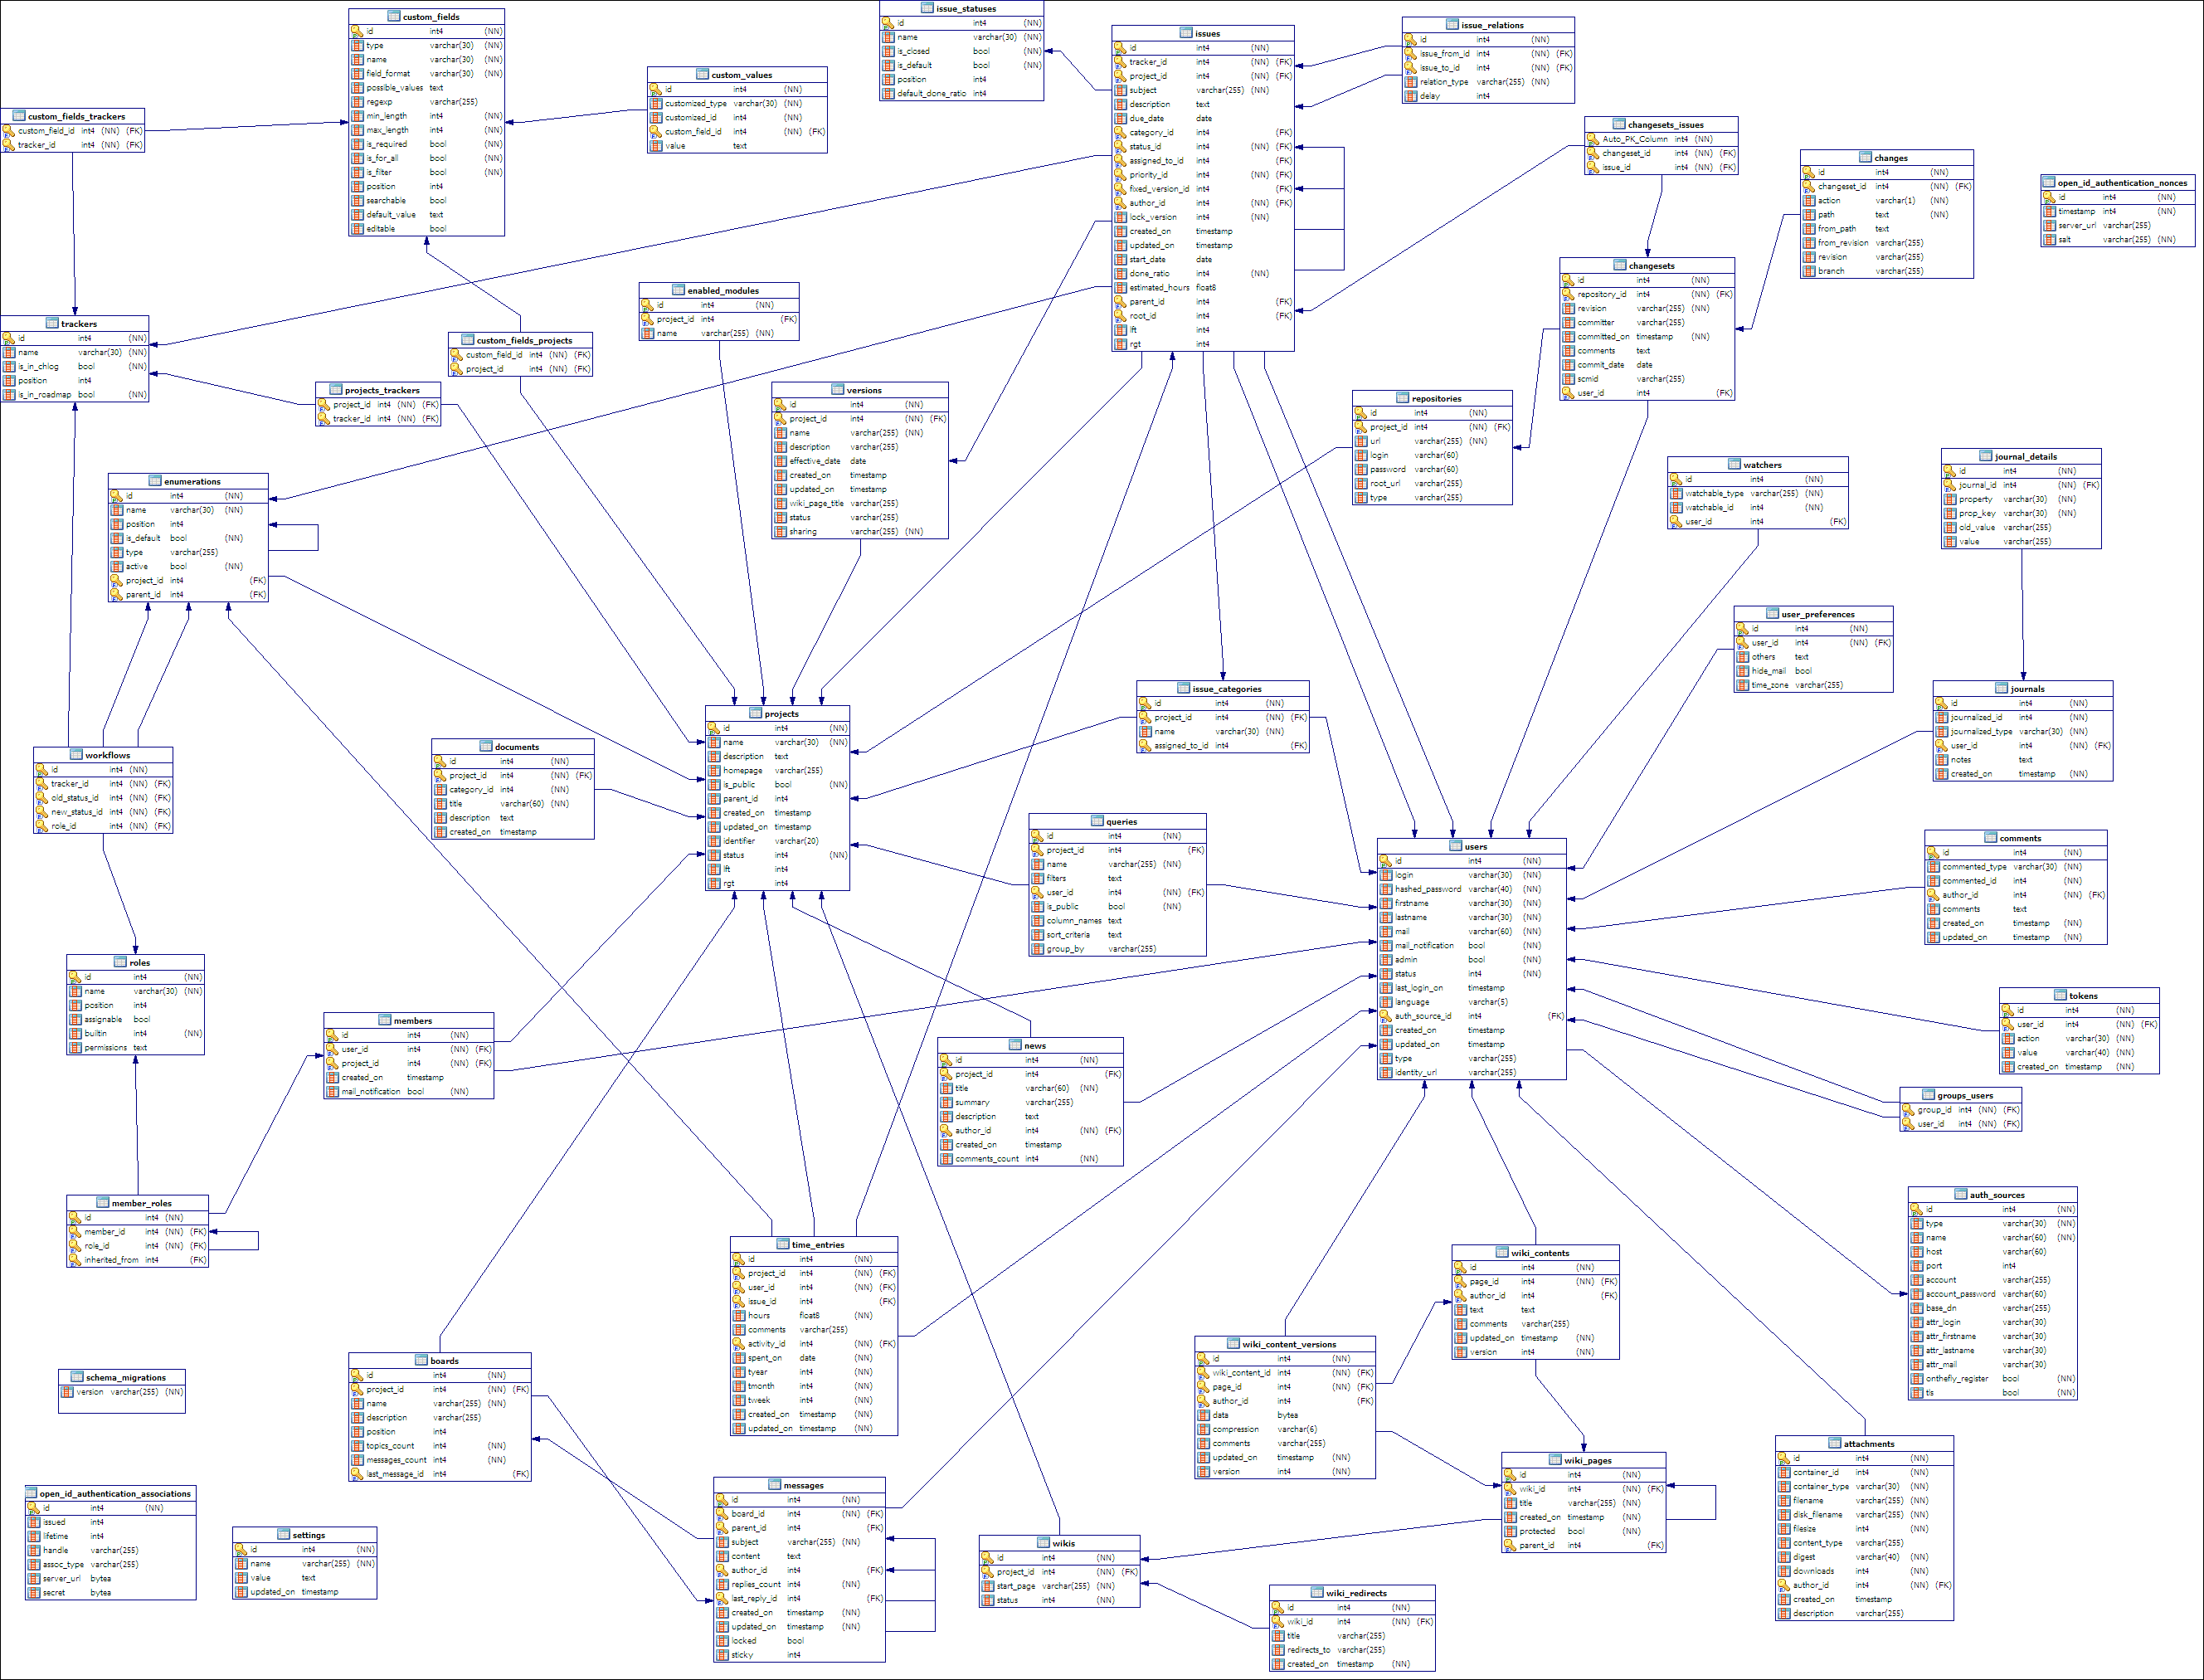
\includegraphics[width=1\textwidth]{img/redmine_er_diagram.png}
	\caption{ER-Диаграмма сервиса redmine}
	\label{fig:redmine-er}
\end{figure}

Исходя из диаграммы выделяются следующие основные сущности:
\begin{itemize}
    \item ядро системы --- проекты, пользователи, задачи;
    \item управление доступом и ролями;
    \item отслеживание изменений и версионирование;
    \item документооборот и вики;
    \item коммуникации --- форумы, новости, комментарии;
    \item учет времени;
    \item настраиваемые поля.
\end{itemize}
В последующих подглавах, будет декомпозированы описанные сущности.

\subsubsection{Сущность \texttt{projects}}
В системе управления проектами redmine проект является основной сущностью она содержит в себе следующую информацию:
\begin{itemize}
    \item \texttt{id} --- уникальный идентификатор проекта;
    \item \texttt{name} --- наименование проекта;
    \item \texttt{description} --- текстовое описание проекта;
    \item \texttt{homepage} --- URL домашней страницы проекта;
    \item \texttt{is\_public} --- флаг публичности проекта;
    \item \texttt{parent\_id} --- идентификатор родительского проекта;
    \item \texttt{created\_on} --- дата создания проекта;
    \item \texttt{updated\_on} --- дата последнего обновления;
    \item \texttt{status} --- статус проекта (активен/архивирован);
    \item \texttt{identifier} --- уникальный текстовый идентификатор проекта;
    % \item \texttt{lft}, \texttt{rgt} --- поля для реализации иерархической структуры.
\end{itemize}

Благодаря полю \texttt{parent\_id}, появляется возможность создавать иерархию проектов.

\subsubsection{Сущность \texttt{users}}

Таблица \texttt{users} хранит информацию о пользователях системы, и содержит в себе следующие поля:
\begin{itemize}
    \item \texttt{id} --- уникальный идентификатор пользователя;
    \item \texttt{login} --- логин пользователя;
    \item \texttt{hashed\_password} --- хешированный пароль;
    \item \texttt{firstname}, \texttt{lastname} --- имя и фамилия;
    \item \texttt{mail} --- адрес электронной почты;
    \item \texttt{admin} --- флаг администратора системы;
    \item \texttt{status} --- статус пользователя (активен/заблокирован);
    \item \texttt{last\_login\_on} --- время последнего входа;
    \item \texttt{created\_on}, \texttt{updated\_on} --- временные метки создания и обновления;
\end{itemize}

\subsubsection{Сущность \texttt{issues}}

Таблица \texttt{issues} представляет основную рабочую единицу системы --- задачу:
\begin{itemize}
    \item \texttt{id} --- уникальный идентификатор задачи;
    \item \texttt{tracker\_id} --- тип задачи;
    \item \texttt{project\_id} --- проект, к которому относится задача;
    \item \texttt{subject} --- название задачи;
    \item \texttt{description} --- описание задачи;
    \item \texttt{due\_date} --- дедлайн;
    \item \texttt{category\_id} --- категория задачи;
    \item \texttt{status\_id} --- статус задачи;
    \item \texttt{assigned\_to\_id} --- исполнитель задачи --- внешний ключ к \texttt{users};
    \item \texttt{priority\_id} --- приоритет задачи;
    \item \texttt{fixed\_version\_id} --- версия, в которой будет исправлена;
    \item \texttt{author\_id} --- автор задачи;
    % \item \texttt{lock\_version} --- версия блокировки для оптимистичной блокировки (integer);
    \item \texttt{created\_on} --- дата создания;
    \item \texttt{updated\_on} --- дата обновления;
    \item \texttt{start\_date} --- дата начала;
    \item \texttt{done\_ratio} --- процент выполнения;
    \item \texttt{estimated\_hours} --- оценочное время в часах;
    \item \texttt{parent\_id} --- родительская задача;
    \item \texttt{root\_id} --- корневая задача в дереве;
    % \item \texttt{lft}, \texttt{rgt} --- поля для древовидной структуры;
    \item \texttt{position} --- позиция в списке.
\end{itemize}

\subsubsection{Сущность \texttt{trackers}}
Таблица \texttt{trackers} определяет типы задач:

\begin{itemize}
    \item \texttt{id} --- идентификатор;
    \item \texttt{name} --- имя типа;
    % \item \texttt{is\_in\_chlog} --- показывать в журнале изменений;
    % \item \texttt{position} --- порядок сортировки (integer);
    % \item \texttt{is\_in\_roadmap} --- показывать в плане работ (boolean).
\end{itemize}

\subsubsection{Сущность \texttt{issue\_statuses}}
Таблица \texttt{issue\_statuses} содержит возможные статусы задач:

\begin{itemize}
    \item \texttt{id} --- идентификатор;
    \item \texttt{name} --- наименование статуса;
    \item \texttt{is\_closed} --- флаг закрытого статуса;
    \item \texttt{is\_default} --- флаг статуса по умолчанию;
    % \item \texttt{position} --- порядок отображения (integer);
    \item \texttt{default\_done\_ratio} --- процент выполнения по умолчанию.
\end{itemize}

\subsubsection{Сущность \texttt{versions}}

Таблица \texttt{versions} хранит информацию о версиях продукта:

\begin{itemize}
    \item \texttt{id} --- идентификатор;
    \item \texttt{project\_id} --- проект, к которому относится версия;
    \item \texttt{name} --- наименование версии;
    \item \texttt{description} --- описание версии;
    \item \texttt{effective\_date} --- планируемая дата релиза;
    \item \texttt{created\_on} --- дата создания;
    \item \texttt{updated\_on} --- дата обновления;
    % \item \texttt{wiki\_page\_title} --- заголовок связанной вики-страницы;
    \item \texttt{status} --- статус версии;
    % \item \texttt{sharing} --- уровень доступа к версии.
\end{itemize}


\subsubsection{Сущность \texttt{roles}}

Таблица \texttt{roles} определяет роли пользователей в системе:

\begin{itemize}
    \item \texttt{id} --- идентификатор;
    \item \texttt{name} --- название роли;
    % \item \texttt{position} --- порядок сортировки;
    \item \texttt{assignable} --- возможность назначения роли;
    % \item \texttt{builtin} --- флаг встроенной роли (integer);
    \item \texttt{permissions} --- текстовое поле с правами доступа.
\end{itemize}

\subsubsection{Сущность \texttt{members}}

Таблица \texttt{members} связывает пользователей с проектами:

\begin{itemize}
    \item \texttt{id} --- уникальный идентификатор;
    \item \texttt{user\_id} --- идентификатор пользователя;
    \item \texttt{project\_id} --- идентификатор проекта;
    \item \texttt{created\_on} --- дата добавления;
    \item \texttt{mail\_notification} --- настройки уведомлений.
\end{itemize}

\subsubsection{Сущность \texttt{custom\_fields} (Настраиваемые поля)}

Таблица \texttt{custom\_fields} определяет пользовательские поля:

\begin{itemize}
    \item \texttt{id} --- идентификатор сущности;
    \item \texttt{type} --- тип поля;
    \item \texttt{name} --- название поля;
    \item \texttt{field\_format} --- формат поля;
    \item \texttt{possible\_values} --- возможные значения;
    % \item \texttt{regexp} --- регулярное выражение для валидации;
    % \item \texttt{min\_length}, \texttt{max\_length} --- ограничения длины (integer);
    \item \texttt{is\_required} --- обязательность заполнения;
    % \item \texttt{is\_for\_all} --- доступно для всех проектов (boolean);
    % \item \texttt{is\_filter} --- использование в фильтрах (boolean);
    % \item \texttt{position} --- порядок отображения;
    \item \texttt{searchable} --- возможность поиска;
    \item \texttt{default\_value} --- значение по умолчанию;
    \item \texttt{editable} --- возможность редактирования.
\end{itemize}

\subsubsection{Остальные сущности}
\begin{itemize}
    \item таблица \texttt{member\_roles} реализует связь многие-ко-многим между участниками и их ролями;
    \item таблица \texttt{watchers} позволяет пользователям подписываться на изменения задач;
\end{itemize}

% \section{Сущности кастомизации}

% \subsection{}


% \subsection{Сущность \texttt{custom\_values} (Значения настраиваемых полей)}

% Таблица \texttt{custom\_values} хранит значения настраиваемых полей:

% \begin{itemize}
%     \item \texttt{id} --- уникальный идентификатор;
%     \item \texttt{customized\_type} --- тип объекта (varchar(30), NOT NULL);
%     \item \texttt{customized\_id} --- идентификатор объекта;
%     \item \texttt{custom\_field\_id} --- ссылка на настраиваемое поле;
%     \item \texttt{value} --- текстовое значение (text).
% \end{itemize}

% \subsection{Сущности \texttt{custom\_fields\_projects} и \texttt{custom\_fields\_trackers}}

% Таблицы связывают настраиваемые поля с конкретными проектами и типами задач:

% \begin{itemize}
%     \item \texttt{custom\_field\_id} --- ссылка на \texttt{custom\_fields};
%     \item \texttt{project\_id} / \texttt{tracker\_id} --- ссылка на проект или тип задачи.
% \end{itemize}

% \section{Сущности отслеживания изменений}

% \subsection{Сущность \texttt{journals} (Журналы изменений)}


% Таблица \texttt{journals} хранит историю изменений задач:

% \begin{itemize}
%     \item \texttt{id} --- уникальный идентификатор;
%     \item \texttt{journable\_id} --- идентификатор изменяемого объекта;
%     \item \texttt{journable\_type} --- тип объекта (varchar(30), NOT NULL);
%     \item \texttt{user\_id} --- пользователь, внесший изменения;
%     \item \texttt{notes} --- текстовые заметки (text);
%     \item \texttt{created\_on} --- дата изменения (timestamp).
% \end{itemize}

% \subsection{Сущность \texttt{journal\_details} (Детали изменений)}

% Таблица \texttt{journal\_details} содержит детали каждого изменения:

% \begin{itemize}
%     \item \texttt{id} --- уникальный идентификатор;
%     \item \texttt{journal\_id} --- ссылка на журнал изменений;
%     \item \texttt{property} --- свойство объекта (varchar(30));
%     \item \texttt{prop\_key} --- ключ свойства (varchar(30));
%     \item \texttt{old\_value} --- старое значение (varchar(255));
%     \item \texttt{value} --- новое значение (varchar(255)).
% \end{itemize}

% \subsection{Сущность \texttt{changesets} (Изменения в системе контроля версий)}

% Таблица \texttt{changesets} хранит информацию о коммитах:

% \begin{itemize}
%     \item \texttt{id} --- уникальный идентификатор;
%     \item \texttt{repository\_id} --- ссылка на репозиторий;
%     \item \texttt{revision} --- ревизия (varchar(255), NOT NULL);
%     \item \texttt{committer} --- автор коммита (varchar(255));
%     \item \texttt{committed\_on} --- дата коммита (timestamp);
%     \item \texttt{comments} --- комментарий к коммиту (text);
%     \item \texttt{commit\_date} --- дата коммита (date);
%     \item \texttt{scmid} --- идентификатор в SCM (varchar(255));
%     \item \texttt{user\_id} --- связанный пользователь Redmine.
% \end{itemize}

% \subsection{Сущность \texttt{changes} (Изменения файлов)}

% Таблица \texttt{changes} хранит информацию об измененных файлах:

% \begin{itemize}
%     \item \texttt{id} --- уникальный идентификатор;
%     \item \texttt{changeset\_id} --- ссылка на changeset;
%     \item \texttt{action} --- действие (varchar(1), NOT NULL);
%     \item \texttt{path} --- путь к файлу (text, NOT NULL);
%     \item \texttt{from\_path} --- исходный путь (text);
%     \item \texttt{from\_revision} --- исходная ревизия (varchar(255));
%     \item \texttt{revision} --- ревизия (varchar(255));
%     \item \texttt{branch} --- ветка (varchar(255)).
% \end{itemize}

% \subsection{Сущность \texttt{changesets\_issues} (Связь коммитов с задачами)}

% Таблица связывает коммиты с задачами:

% \begin{itemize}
%     \item \texttt{changeset\_id} --- ссылка на changeset;
%     \item \texttt{issue\_id} --- ссылка на задачу.
% \end{itemize}

% \subsection{Сущность \texttt{repositories} (Репозитории)}

% Таблица \texttt{repositories} хранит информацию о репозиториях:

% \begin{itemize}
%     \item \texttt{id} --- уникальный идентификатор;
%     \item \texttt{project\_id} --- проект, к которому относится репозиторий;
%     \item \texttt{url} --- URL репозитория (varchar(255), NOT NULL);
%     \item \texttt{login} --- логин для доступа (varchar(60));
%     \item \texttt{password} --- пароль (varchar(60));
%     \item \texttt{root\_url} --- корневой URL (varchar(255));
%     \item \texttt{type} --- тип репозитория (Git, SVN, Mercurial и т.д.);
%     \item \texttt{is\_default} --- флаг репозитория по умолчанию (boolean).
% \end{itemize}

% \section{Сущности документооборота и вики}

% \subsection{Сущность \texttt{documents} (Документы)}

% Таблица \texttt{documents} хранит метаданные документов:

% \begin{itemize}
%     \item \texttt{id} --- уникальный идентификатор;
%     \item \texttt{project\_id} --- проект документа;
%     \item \texttt{category\_id} --- категория документа;
%     \item \texttt{title} --- заголовок документа (varchar(60), NOT NULL);
%     \item \texttt{description} --- описание (text);
%     \item \texttt{created\_on} --- дата создания (timestamp).
% \end{itemize}

% \subsection{Сущность \texttt{attachments} (Вложения)}

% Таблица \texttt{attachments} хранит информацию о вложенных файлах:

% \begin{itemize}
%     \item \texttt{id} --- уникальный идентификатор;
%     \item \texttt{container\_id} --- идентификатор объекта-контейнера;
%     \item \texttt{container\_type} --- тип контейнера (varchar(30), NOT NULL);
%     \item \texttt{filename} --- имя файла (varchar(255), NOT NULL);
%     \item \texttt{disk\_filename} --- имя файла на диске (varchar(255));
%     \item \texttt{filesize} --- размер файла (integer);
%     \item \texttt{content\_type} --- MIME-тип (varchar(255));
%     \item \texttt{digest} --- хеш файла (varchar(40), NOT NULL);
%     \item \texttt{downloads} --- количество скачиваний (integer, NOT NULL);
%     \item \texttt{author\_id} --- автор загрузки;
%     \item \texttt{created\_on} --- дата загрузки (timestamp);
%     \item \texttt{description} --- описание файла (varchar(255)).
% \end{itemize}

% \subsection{Сущность \texttt{wikis} (Вики-проекты)}

% Таблица \texttt{wikis} определяет вики для проектов:

% \begin{itemize}
%     \item \texttt{id} --- уникальный идентификатор;
%     \item \texttt{project\_id} --- проект вики (NOT NULL);
%     \item \texttt{start\_page} --- стартовая страница (varchar(255), NOT NULL);
%     \item \texttt{status} --- статус вики (integer).
% \end{itemize}

% \subsection{Сущность \texttt{wiki\_pages} (Страницы вики)}

% Таблица \texttt{wiki\_pages} содержит информацию о страницах:

% \begin{itemize}
%     \item \texttt{id} --- уникальный идентификатор;
%     \item \texttt{wiki\_id} --- ссылка на вики-проект;
%     \item \texttt{title} --- заголовок страницы (varchar(255), NOT NULL, уникальный);
%     \item \texttt{created\_on} --- дата создания (timestamp);
%     \item \texttt{protected} --- флаг защищенной страницы (boolean);
%     \item \texttt{parent\_id} --- родительская страница.
% \end{itemize}

% \subsection{Сущность \texttt{wiki\_contents} (Содержимое вики-страниц)}

% Таблица \texttt{wiki\_contents} хранит текст страниц:

% \begin{itemize}
%     \item \texttt{id} --- уникальный идентификатор;
%     \item \texttt{page\_id} --- ссылка на страницу;
%     \item \texttt{author\_id} --- автор содержимого;
%     \item \texttt{text} --- текст страницы (mediumtext);
%     \item \texttt{comments} --- комментарий к редакции (varchar(255));
%     \item \texttt{updated\_on} --- дата обновления (timestamp);
%     \item \texttt{version} --- номер версии (integer, NOT NULL).
% \end{itemize}

% \subsection{Сущность \texttt{wiki\_content\_versions} (Версии вики-содержимого)}

% Таблица \texttt{wiki\_content\_versions} хранит историю изменений:

% \begin{itemize}
%     \item \texttt{id} --- уникальный идентификатор;
%     \item \texttt{wiki\_content\_id} --- ссылка на содержимое;
%     \item \texttt{page\_id} --- ссылка на страницу;
%     \item \texttt{author\_id} --- автор;
%     \item \texttt{data} --- бинарные данные (bytes);
%     \item \texttt{compression} --- метод сжатия (varchar(6));
%     \item \texttt{comments} --- комментарий (varchar(255));
%     \item \texttt{updated\_on} --- дата обновления (timestamp);
%     \item \texttt{version} --- номер версии (integer, NOT NULL).
% \end{itemize}

% \section{Сущности коммуникаций}

% \subsection{Сущность \texttt{news} (Новости)}

% Таблица \texttt{news} хранит новостные сообщения проектов:

% \begin{itemize}
%     \item \texttt{id} --- уникальный идентификатор;
%     \item \texttt{project\_id} --- проект новости;
%     \item \texttt{title} --- заголовок (varchar(60), NOT NULL);
%     \item \texttt{summary} --- краткое содержание (varchar(255));
%     \item \texttt{description} --- полное описание (text);
%     \item \texttt{author\_id} --- автор новости;
%     \item \texttt{created\_on} --- дата создания (timestamp);
%     \item \texttt{comments\_count} --- количество комментариев (integer).
% \end{itemize}

% \subsection{Сущность \texttt{boards} (Форумы)}

% Таблица \texttt{boards} определяет форумы проектов:

% \begin{itemize}
%     \item \texttt{id} --- уникальный идентификатор;
%     \item \texttt{project\_id} --- проект форума;
%     \item \texttt{name} --- название форума (varchar(255), NOT NULL);
%     \item \texttt{description} --- описание (varchar(255));
%     \item \texttt{position} --- порядок отображения (integer);
%     \item \texttt{topics\_count} --- количество тем (integer);
%     \item \texttt{messages\_count} --- количество сообщений (integer);
%     \item \texttt{last\_message\_id} --- последнее сообщение.
% \end{itemize}

% \subsection{Сущность \texttt{messages} (Сообщения форумов)}

% Таблица \texttt{messages} хранит сообщения форумов:

% \begin{itemize}
%     \item \texttt{id} --- уникальный идентификатор;
%     \item \texttt{board\_id} --- форум сообщения;
%     \item \texttt{parent\_id} --- родительское сообщение (для тредов);
%     \item \texttt{subject} --- тема сообщения (varchar(255), NOT NULL);
%     \item \texttt{content} --- содержимое (text);
%     \item \texttt{author\_id} --- автор сообщения;
%     \item \texttt{replies\_count} --- количество ответов (integer);
%     \item \texttt{last\_reply\_id} --- последний ответ;
%     \item \texttt{created\_on}, \texttt{updated\_on} --- временные метки;
%     \item \texttt{locked} --- флаг заблокированной темы (boolean);
%     \item \texttt{sticky} --- флаг закрепленной темы (integer).
% \end{itemize}

% \subsection{Сущность \texttt{comments} (Комментарии)}

% Таблица \texttt{comments} хранит комментарии к различным объектам:

% \begin{itemize}
%     \item \texttt{id} --- уникальный идентификатор;
%     \item \texttt{commented\_type} --- тип комментируемого объекта (varchar(30), NOT NULL);
%     \item \texttt{commented\_id} --- идентификатор объекта;
%     \item \texttt{author\_id} --- автор комментария;
%     \item \texttt{comments} --- текст комментария (text, NOT NULL);
%     \item \texttt{created\_on}, \texttt{updated\_on} --- временные метки.
% \end{itemize}

% \section{Сущности учета времени}

% \subsection{Сущность \texttt{time\_entries} (Учет времени)}

% Таблица \texttt{time\_entries} фиксирует затраченное время:

% \begin{itemize}
%     \item \texttt{id} --- уникальный идентификатор;
%     \item \texttt{project\_id} --- проект;
%     \item \texttt{user\_id} --- пользователь;
%     \item \texttt{issue\_id} --- задача (может быть NULL);
%     \item \texttt{hours} --- количество часов (float(8,6), NOT NULL);
%     \item \texttt{comments} --- комментарий (varchar(255));
%     \item \texttt{activity\_id} --- тип активности;
%     \item \texttt{spent\_on} --- дата работы (date, NOT NULL);
%     \item \texttt{tweek} --- неделя (integer);
%     \item \texttt{tmonth} --- месяц (integer);
%     \item \texttt{tyear} --- год (integer);
%     \item \texttt{created\_on}, \texttt{updated\_on} --- временные метки.
% \end{itemize}

% \section{Вспомогательные и справочные сущности}

% \subsection{Сущность \texttt{enumerations} (Перечисления)}

% Таблица \texttt{enumerations} хранит справочные значения:

% \begin{itemize}
%     \item \texttt{id} --- уникальный идентификатор;
%     \item \texttt{name} --- наименование (varchar(30), NOT NULL);
%     \item \texttt{position} --- порядок (integer);
%     \item \texttt{is\_default} --- значение по умолчанию (boolean);
%     \item \texttt{type} --- тип перечисления (varchar(255));
%     \item \texttt{active} --- флаг активности (boolean);
%     \item \texttt{project\_id} --- проект (NULL для глобальных);
%     \item \texttt{parent\_id} --- родительское значение.
% \end{itemize}

% Типы перечислений: IssuePriority (приоритеты), DocumentCategory (категории документов), TimeEntryActivity (виды деятельности).

% \subsection{Сущность \texttt{issue\_categories} (Категории задач)}

% Таблица \texttt{issue\_categories} определяет категории задач:

% \begin{itemize}
%     \item \texttt{id} --- уникальный идентификатор;
%     \item \texttt{project\_id} --- проект категории;
%     \item \texttt{name} --- название категории (varchar(255), NOT NULL);
%     \item \texttt{assigned\_to\_id} --- ответственный по умолчанию.
% \end{itemize}

% \subsection{Сущность \texttt{issue\_relations} (Связи задач)}

% Таблица \texttt{issue\_relations} определяет связи между задачами:

% \begin{itemize}
%     \item \texttt{id} --- уникальный идентификатор;
%     \item \texttt{issue\_from\_id} --- исходная задача;
%     \item \texttt{issue\_to\_id} --- целевая задача;
%     \item \texttt{relation\_type} --- тип связи (varchar(255), NOT NULL);
%     \item \texttt{delay} --- задержка в днях (integer).
% \end{itemize}

% Типы связей: relates, duplicates, blocks, precedes, follows.

% \subsection{Сущность \texttt{queries} (Сохраненные запросы)}

% Таблица \texttt{queries} хранит пользовательские фильтры:

% \begin{itemize}
%     \item \texttt{id} --- уникальный идентификатор;
%     \item \texttt{project\_id} --- проект (NULL для глобальных);
%     \item \texttt{name} --- название запроса (varchar(255), NOT NULL);
%     \item \texttt{filters} --- условия фильтрации (text);
%     \item \texttt{user\_id} --- автор запроса;
%     \item \texttt{is\_public} --- публичный доступ (boolean);
%     \item \texttt{column\_names} --- отображаемые колонки (text);
%     \item \texttt{sort\_criteria} --- критерии сортировки (text);
%     \item \texttt{group\_by} --- группировка (varchar(255)).
% \end{itemize}

% \subsection{Сущность \texttt{workflows} (Рабочие процессы)}

% Таблица \texttt{workflows} определяет правила перехода статусов:

% \begin{itemize}
%     \item \texttt{id} --- уникальный идентификатор;
%     \item \texttt{tracker\_id} --- тип задачи;
%     \item \texttt{old\_status\_id} --- текущий статус;
%     \item \texttt{new\_status\_id} --- новый статус;
%     \item \texttt{role\_id} --- роль;
%     \item \texttt{assignee} --- разрешено ли назначение.
% \end{itemize}

% \subsection{Сущность \texttt{user\_preferences} (Настройки пользователя)}

% Таблица \texttt{user\_preferences} хранит предпочтения пользователей:

% \begin{itemize}
%     \item \texttt{id} --- уникальный идентификатор;
%     \item \texttt{user\_id} --- пользователь;
%     \item \texttt{others} --- дополнительные настройки (text);
%     \item \texttt{hide\_mail} --- скрыть email (boolean);
%     \item \texttt{time\_zone} --- часовой пояс (varchar(255)).
% \end{itemize}

% \subsection{Сущность \texttt{settings} (Настройки системы)}

% Таблица \texttt{settings} содержит глобальные настройки:

% \begin{itemize}
%     \item \texttt{id} --- уникальный идентификатор;
%     \item \texttt{name} --- наименование настройки (varchar(255), NOT NULL);
%     \item \texttt{value} --- значение (text);
%     \item \texttt{updated\_on} --- дата обновления (timestamp).
% \end{itemize}

% \subsection{Сущность \texttt{enabled\_modules} (Включенные модули)}

% Таблица \texttt{enabled\_modules} определяет активные модули проектов:

% \begin{itemize}
%     \item \texttt{id} --- уникальный идентификатор;
%     \item \texttt{project\_id} --- проект;
%     \item \texttt{name} --- название модуля (varchar(255), NOT NULL).
% \end{itemize}

% \subsection{Сущность \texttt{tokens} (Токены)}

% Таблица \texttt{tokens} хранит токены для различных операций:

% \begin{itemize}
%     \item \texttt{id} --- уникальный идентификатор;
%     \item \texttt{user\_id} --- пользователь;
%     \item \texttt{action} --- действие (varchar(30), NOT NULL);
%     \item \texttt{value} --- значение токена (varchar(40), NOT NULL);
%     \item \texttt{created\_on} --- дата создания (timestamp).
% \end{itemize}

% \subsection{Сущность \texttt{auth\_sources} (Источники аутентификации)}

% Таблица \texttt{auth\_sources} настраивает внешнюю аутентификацию:

% \begin{itemize}
%     \item \texttt{id} --- уникальный идентификатор;
%     \item \texttt{type} --- тип (varchar(30), NOT NULL);
%     \item \texttt{name} --- наименование (varchar(30), NOT NULL);
%     \item \texttt{host} --- хост (varchar(60));
%     \item \texttt{port} --- порт (integer);
%     \item \texttt{account} --- учетная запись (varchar(255));
%     \item \texttt{account\_password} --- пароль (varchar(60));
%     \item \texttt{base\_dn} --- базовый DN (varchar(255));
%     \item \texttt{attr\_login}, \texttt{attr\_firstname}, \texttt{attr\_lastname}, \texttt{attr\_mail} --- атрибуты LDAP;
%     \item \texttt{onthefly\_register} --- регистрация на лету (boolean);
%     \item \texttt{tls} --- использование TLS (boolean).
% \end{itemize}

% \subsection{Сущность \texttt{groups\_users} (Группы пользователей)}

% Таблица связывает группы с пользователями:

% \begin{itemize}
%     \item \texttt{group\_id} --- идентификатор группы;
%     \item \texttt{user\_id} --- идентификатор пользователя.
% \end{itemize}

% \subsection{Сущность \texttt{schema\_migrations} (Миграции схемы)}

% Таблица \texttt{schema\_migrations} отслеживает версии миграций БД:

% \begin{itemize}
%     \item \texttt{version} --- версия миграции (varchar(255), NOT NULL).
% \end{itemize}

% \section{Анализ связей между сущностями}

% \subsection{Основные отношения}

% Архитектура базы данных Redmine реализует следующие типы отношений:

% \begin{enumerate}
%     \item \textbf{Один-ко-многим}: 
%     \begin{itemize}
%         \item \texttt{projects} $\rightarrow$ \texttt{issues} (один проект содержит много задач);
%         \item \texttt{users} $\rightarrow$ \texttt{issues} (один пользователь может быть автором многих задач);
%         \item \texttt{trackers} $\rightarrow$ \texttt{issues} (один тип задачи используется во многих задачах).
%     \end{itemize}
    
%     \item \textbf{Многие-ко-многим}:
%     \begin{itemize}
%         \item \texttt{users} $\leftrightarrow$ \texttt{projects} через \texttt{members};
%         \item \texttt{members} $\leftrightarrow$ \texttt{roles} через \texttt{member\_roles};
%         \item \texttt{issues} $\leftrightarrow$ \texttt{changesets} через \texttt{changesets\_issues}.
%     \end{itemize}
    
%     \item \textbf{Рекурсивные отношения}:
%     \begin{itemize}
%         \item \texttt{issues}.\texttt{parent\_id} $\rightarrow$ \texttt{issues}.\texttt{id} (иерархия задач);
%         \item \texttt{projects}.\texttt{parent\_id} $\rightarrow$ \texttt{projects}.\texttt{id} (иерархия проектов);
%         \item \texttt{messages}.\texttt{parent\_id} $\rightarrow$ \texttt{messages}.\texttt{id} (треды форумов).
%     \end{itemize}
% \end{enumerate}

% \subsection{Целостность данных}

% Система обеспечивает целостность данных через:

% \begin{itemize}
%     \item внешние ключи (Foreign Keys) с каскадным удалением;
%     \item ограничения NOT NULL для обязательных полей;
%     \item уникальные индексы для ключевых полей;
%     \item оптимистичную блокировку через поле \texttt{lock\_version}.
% \end{itemize}

% \section{Выводы}

% База данных Redmine представляет собой хорошо структурированную реляционную модель, охватывающую все аспекты управления проектами:

% \begin{enumerate}
%     \item \textbf{Модульность}: система разделена на логические модули (задачи, вики, документы, форумы), которые могут быть независимо включены/выключены.
    
%     \item \textbf{Гибкость}: механизм настраиваемых полей позволяет адаптировать систему под специфические требования проектов.
    
%     \item \textbf{Отслеживаемость}: полная история изменений через журналы (\texttt{journals}, \texttt{journal\_details}) и интеграция с системами контроля версий.
    
%     \item \textbf{Масштабируемость}: поддержка иерархических структур проектов и задач позволяет работать с крупными проектами.
    
%     \item \textbf{Безопасность}: многоуровневая система ролей и прав доступа, поддержка внешней аутентификации (LDAP).
    
%     \item \textbf{Коммуникация}: встроенные инструменты коммуникации (форумы, новости, комментарии, уведомления).
% \end{enumerate}

% Такая архитектура обеспечивает надежное хранение данных, эффективное выполнение запросов и возможность расширения функциональности системы.

% \begin{enumerate}
% \item \textbf{Пользователь (User)} — субъект, взаимодействующий с системой.
% \item \textbf{Проект (Project)} — контейнер для задач, версий и документов.
% \item \textbf{Задача (Issue)} — единица работы, требующая выполнения.
% \item \textbf{Версия (Version)} — релиз или веха проекта.
% \item \textbf{Репозиторий (Repository)} — связь с внешней системой контроля версий.
% \item \textbf{Журнал изменений (Journal)} — история модификации сущностей.
% \end{enumerate}
% \section{Описание атрибутов сущностей}
% Ниже приведены таблицы с описанием полей для каждой выделенной сущности. Типы данных указаны в соответствии с распространенными СУБД (MySQL/PostgreSQL), используемыми в Redmine.
% \subsection{Сущность \texttt{users}}
% Данная таблица хранит учетные данные и профильную информацию о пользователях системы.
% \begin{table}[h!]
% \centering
% \caption{Атрибуты сущности \texttt{users}}
% \label{tab:users}
% \begin{tabular}{lll}
% \toprule
% \textbf{Поле} & \textbf{Тип данных} & \textbf{Описание} \
% \midrule
% \texttt{id} & INTEGER (PK) & Уникальный идентификатор пользователя \
% \texttt{login} & VARCHAR(255) & Уникальное имя для входа \
% \texttt{password_hash} & VARCHAR(64) & Хэш пароля \
% \texttt{firstname} & VARCHAR(255) & Имя \
% \texttt{lastname} & VARCHAR(255) & Фамилия \
% \texttt{mail} & VARCHAR(255) & Адрес электронной почты \
% \texttt{admin} & BOOLEAN & Флаг администратора \
% \texttt{status} & INTEGER & Статус активности (активен/блокирован) \
% \texttt{created_on} & DATETIME & Дата создания записи \
% \bottomrule
% \end{tabular}
% \end{table}
% \subsection{Сущность \texttt{projects}}
% Таблица содержит информацию о проектах, включая их иерархию и статус.
% \begin{table}[h!]
% \centering
% \caption{Атрибуты сущности \texttt{projects}}
% \label{tab:projects}
% \begin{tabular}{lll}
% \toprule
% \textbf{Поле} & \textbf{Тип данных} & \textbf{Описание} \
% \midrule
% \texttt{id} & INTEGER (PK) & Уникальный идентификатор проекта \
% \texttt{name} & VARCHAR(255) & Название проекта \
% \texttt{identifier} & VARCHAR(255) & Уникальный URL-идентификатор \
% \texttt{description} & TEXT & Подробное описание \
% \texttt{parent_id} & INTEGER (FK) & Ссылка на родительский проект \
% \texttt{status} & INTEGER & Статус проекта (активен/закрыт) \
% \texttt{created_on} & DATETIME & Дата создания \
% \bottomrule
% \end{tabular}
% \end{table}
% \subsection{Сущность \texttt{issues}}
% Центральная сущность системы, представляющая задачу или ошибку.
% \begin{table}[h!]
% \centering
% \caption{Атрибуты сущности \texttt{issues}}
% \label{tab:issues}
% \begin{tabular}{lll}
% \toprule
% \textbf{Поле} & \textbf{Тип данных} & \textbf{Описание} \
% \midrule
% \texttt{id} & INTEGER (PK) & Уникальный идентификатор задачи \
% \texttt{project_id} & INTEGER (FK) & Ссылка на проект \
% \texttt{tracker_id} & INTEGER (FK) & Тип задачи (баг, функция и т.д.) \
% \texttt{status_id} & INTEGER (FK) & Текущий статус задачи \
% \texttt{author_id} & INTEGER (FK) & Автор задачи \
% \texttt{assigned_to_id} & INTEGER (FK) & Исполнитель задачи \
% \texttt{subject} & VARCHAR(255) & Краткая тема задачи \
% \texttt{description} & TEXT & Подробное описание \
% \texttt{priority_id} & INTEGER (FK) & Приоритет выполнения \
% \texttt{fixed_version_id} & INTEGER (FK) & Целевая версия для задачи \
% \texttt{created_on} & DATETIME & Дата создания \
% \texttt{updated_on} & DATETIME & Дата последнего обновления \
% \bottomrule
% \end{tabular}
% \end{table}
% \subsection{Сущность \texttt{versions}}
% Определяет релизы или вехи проекта, к которым могут быть привязаны задачи.
% \begin{table}[h!]
% \centering
% \caption{Атрибуты сущности \texttt{versions}}
% \label{tab:versions}
% \begin{tabular}{lll}
% \toprule
% \textbf{Поле} & \textbf{Тип данных} & \textbf{Описание} \
% \midrule
% \texttt{id} & INTEGER (PK) & Уникальный идентификатор версии \
% \texttt{project_id} & INTEGER (FK) & Ссылка на проект \
% \texttt{name} & VARCHAR(255) & Название версии (например, 1.0.0) \
% \texttt{description} & TEXT & Описание версии \
% \texttt{status} & VARCHAR(255) & Статус (открыта, закрыта, заблокирована) \
% \texttt{due_date} & DATE & Планируемая дата релиза \
% \texttt{created_on} & DATETIME & Дата создания \
% \bottomrule
% \end{tabular}
% \end{table}
% \subsection{Сущность \texttt{repositories}}
% Обеспечивает интеграцию с внешними системами контроля версий (Git, SVN).
% \begin{table}[h!]
% \centering
% \caption{Атрибуты сущности \texttt{repositories}}
% \label{tab:repositories}
% \begin{tabular}{lll}
% \toprule
% \textbf{Поле} & \textbf{Тип данных} & \textbf{Описание} \
% \midrule
% \texttt{id} & INTEGER (PK) & Уникальный идентификатор репозитория \
% \texttt{project_id} & INTEGER (FK) & Ссылка на проект \
% \texttt{url} & VARCHAR(255) & Путь к репозиторию \
% \texttt{login} & VARCHAR(255) & Логин для доступа (если требуется) \
% \texttt{password} & VARCHAR(255) & Пароль для доступа (зашифрованный) \
% \texttt{root_url} & VARCHAR(255) & Корневой URL для веб-доступа \
% \texttt{type} & VARCHAR(255) & Тип VCS (Git, Subversion, Mercurial) \
% \bottomrule
% \end{tabular}
% \end{table}
% \section{Заключение по главе}
Проведенный анализ сущностей системы Redmine позволяет выделить ключевые компоненты, необходимые для построения базы данных системы управления разработкой. Основные связи между сущностями реализуются через внешние ключи (Foreign Keys), обеспечивая целостность данных. Например, сущность \texttt{issues} связана с \texttt{projects}, \texttt{users} и \texttt{versions}, что отражает логику бизнес-процесса: задача создается пользователем в рамках проекта и планируется к определенной версии.

\subsection[Описание типовых процессов и ролей в redmine, связанные с учебным процессом]{Описание типовых процессов и ролей в redmine, связанные с учебным процессом}
В текущем учебном процессе можно выделить следующие сущности:
\begin{itemize}
    \item задача;
    \item система управления проектами;
    \item студент;
    \item преподаватель;
    \item система управления проектами (gitlab).
\end{itemize}

Объекты, которые взаимодействует с данными сущностями:
\begin{itemize}
    \item генератор задач;
    \item администратор системы управления проектами;
    \item скрипт для создания задач в системе управления проктами;
    \item TODO gitlab bot. 
\end{itemize}

Были выделены следубщие процессы:
\begin{enumerate}
    \item генерация задачи и запись ее в базу данных задач.
    \item \textbf{Администратор СУП:} запуск сервиса на сервере, создание пользователей, настройка трекеров и статусов, создание проекта, добавление пользователей в проект. 
    \item \textbf{Создание задачи:} скрипт достает задачу из базы данных и добавляет ее в систему управления проектами.
    \item \textbf{Выполнение задачи:}
    \item \textbf{Проверка задачи:}
\end{enumerate}

На основании текущего учебного процесса была построена BPMN 2.0 диаграмма, представленная на рисунке~\ref{fig:bpmn-1}
\begin{figure}[H]
	\centering
	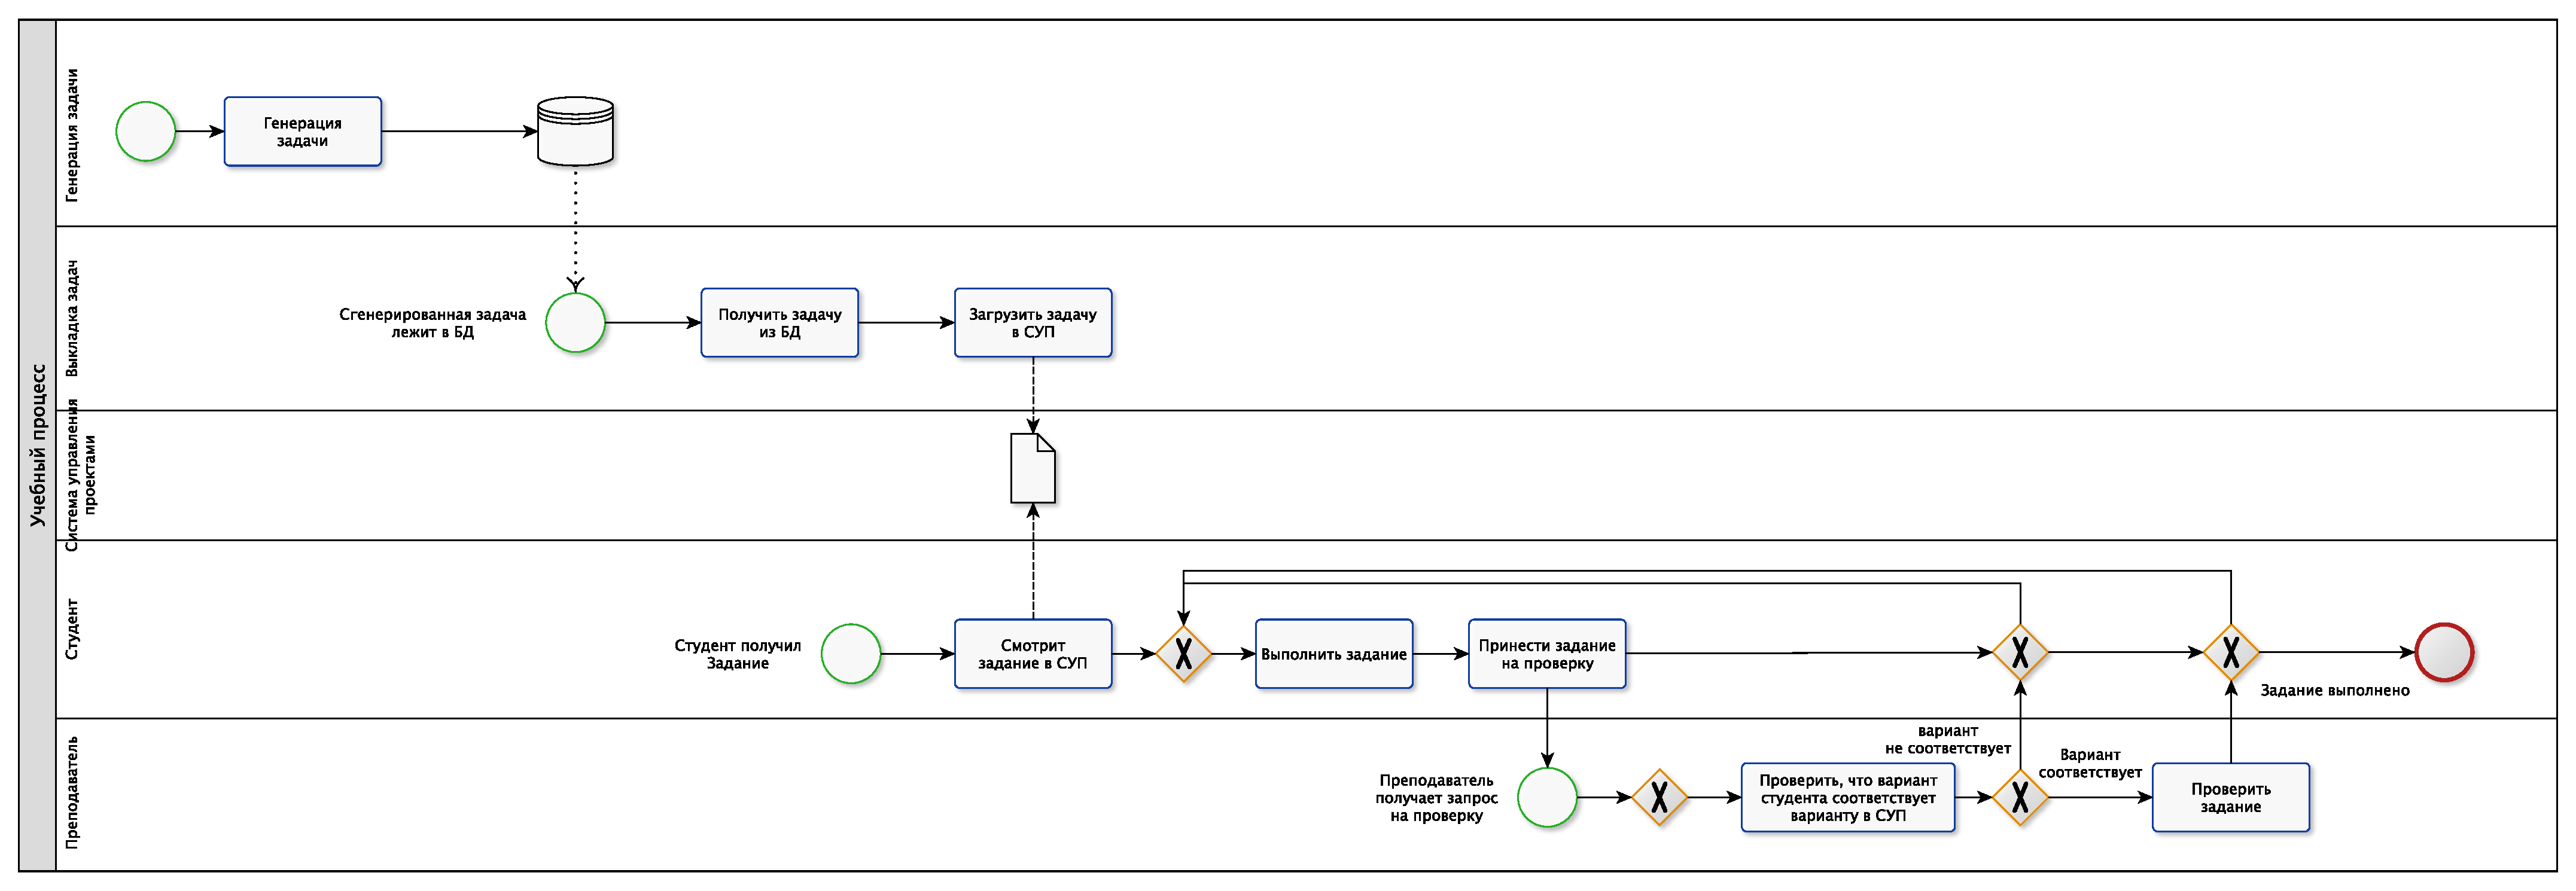
\includegraphics[width=1\textwidth]{diag/bpmn-1.pdf}
	\caption{Диаграмма BPMN-2.0 учебного процесса}
	\label{fig:bpmn-1}
\end{figure}

\subsubsection{Процесс выдачи задачи}
TODO


\subsection[Анализ существующих решений в области СУБД]{Анализ существующих решений в области \\ СУБД}
Система управления базами данных (СУБД) --- приложение, обеспечивающее создание, хранение, обновление и поиск информации в базах данных.
СУБД классифицируются следующими по нескольким признакам:
\begin{itemize}
\item \textbf{по модели данных}: иерархическая, сетевая, документоориентированная, реляционная, объектно-ориентированная, колоночная, графовая;
\item \textbf{по архитектуре организации хранения данных}: локальные, распределённые;
\item \textbf{по способу доступа к данным}: файл-серверные, встраиваемые, клиент-серверные, сервисно-ориентированные.
\end{itemize}

В данном разделе будет приведена информация о моделях данных в базах данных.


\subsubsection{Иерархическая модель данных}
Иерархическая модель данных стала первой широко распространенной моделью организации данных в коммерческих СУБД.
Данные представляются в виде дерева.
Связи между данными реализуются через физические указатели и представляют собой отношения типа «один-ко-многим».

Иерархическая модель используется для отображения иерархической структуры работ.
Доступ к данным осуществляется путем навигации от корня дерева вниз по уровням вложенности.
При работе с иерархическими базами данных выделяют следующие приемущества и недостатки: \\
\textbf{преимущества:}
\begin{enumerate}
\item поиск в дереве имеет алгоритмическую сложность $O(log n)$.
\end{enumerate}
\textbf{Недостатки:}
\begin{enumerate}
\item невозможна реализации связи «многие-ко-многим» без дублирования данных.
\end{enumerate}

\subsubsection{Сетевая модель данных}
Сетевая модель данных~\cite{network-db} была разработана как расширение иерархической модели для устранения ее основных недостатков.
В сетевой модели запись может иметь несколько родителей, что позволяет организовывать данные в виде произвольного графа.
Данные организовуются в виде наборов, состоящих из владельца и членов.
У сетевой модели данных можно выделить следующие примущества и недостатки: \\
\textbf{преимущества:}
\begin{enumerate}
\item возможность представления отношения «многие-ко-многим».
\end{enumerate}
\textbf{Недостатки:}
\begin{enumerate}
\item устаревание технологии.
\end{enumerate}


\subsubsection{Реляционная модель данных}
В настоящее время реляционная модель данных, предложенная Э.Ф. Коддом в 1970 году, является доминирующей на рынке СУБД~\cite{relation-bd-research}.
Данные представляются в виде набора отношений (таблиц), каждое из которых состоит из строк (кортежей) и столбцов (атрибутов).
В реляционных СУБД связи между таблицами устанавливаются логически с помощью первичных и вторичных ключей.
\begin{itemize}
\item \textbf{Первичный ключ (Primary Key):} уникально идентифицирует запись в таблице.
\item \textbf{Внешний ключ (Foreign Key):} ссылается на первичный ключ другой таблицы, обеспечивая ссылочную целостность.
\end{itemize}

Для взаимодействия используется структурированный язык запросов SQL (Structured Query Language),
который состоит из следующих языков:
\begin{itemize}
    \item \textbf{DDL} (Data Definition Language) определяет структуру базы данных, позволяя создавать, изменять и удалять объекты.
    \item \textbf{DML} (Data Manipulation Language) управляет содержимым таблиц, обеспечивая вставку, обновление и удаление записей.
    \item \textbf{DQL} (Data Query Language) предназначен исключительно для выборки и чтения данных из базы без их изменения.
    \item \textbf{DCL} (Data Control Language) регулирует права доступа пользователей к объектам базы данных с помощью команд предоставления и отзыва привилегий.
    \item \textbf{TCL} (Transaction Control Language) контролирует целостность транзакций, позволяя подтверждать или откатывать группы операций.
\end{itemize}
Реляционный базы данных обладают фундаментальными свойствами ACID, которые помогают избежать неопределенного поведения при работе с данными:
\begin{itemize}
    \item \textbf{Atomicity} (Атомарность): Транзакция выполняется целиком или не выполняется вовсе; не допускается частичное выполнение.
    \item \textbf{Consistency} (Согласованность): Транзакция переводит базу данных из одного согласованного состояния в другое, сохраняя целостность данных.
    \item \textbf{Isolation} (Изолированность): Параллельные транзакции не влияют друг на друга, обеспечивая независимость выполнения.
    \item \textbf{Durability} (Долговечность): Успешно завершенная транзакция сохраняется даже при сбоях оборудования. 
\end{itemize}
У реляционных баз данных выделяют следующие примущества и недостатки:
\textbf{преимущества:}
\begin{enumerate}
\item \textbf{целостность данных (ACID):} свойства ACID обеспечивают базе данных целостность данных, помогая избегать конфликтов;
\item \textbf{нормализация:} возможность приведения базы данных к нормальным формам для устранения избыточности и аномалий обновления.
\end{enumerate}
\textbf{Недостатки:}
\begin{enumerate}
\item изменение структуры таблиц на больших объемах данных может блокировать работу системы;
\item при чрезмерной нормализации и большом количестве связей запросы с множественными соединениями выполняются медленнее.
\end{enumerate}

В данный момент наибольшей популярностью пользуются следующие реляционные базы данных: PostgreSQL, MySQL, Oracle, MS SQL Server.

\subsubsection{Документоориентированная модель данных}
Документоориентированные СУБД относятся к классу NoSQL.
Данные хранятся в виде документов, где каждый документ содержит данные в виде пар «ключ-значение» или вложенных структур.
В таких системах (MongoDB, Couchbase, RavenDB) отсутствует жесткая схема данных.
Документы в одной коллекции могут иметь различный набор полей.
Данные часто денормализованы: связанная информация может храниться внутри одного документа.
Выделяют следующие примущества и недостатки:
\textbf{преимущества:}
\begin{enumerate}
\item можно добавлять новые атрибуты к задачам без миграции всей базы данных;
\item высокая скорость вставки данных благодаря отсутствию проверок внешних ключей и транзакционных блокировок на уровне строк.
\end{enumerate}
\textbf{Недостатки:}
\begin{enumerate}
\item \textbf{сложность связей:} реализация связей между документами менее эффективна, чем в реляционной моделе данных;
\item дублирование данных.
\end{enumerate}

\subsubsection{Объектно-ориентированная модель данных}
Объектно-ориентированные СУБД (OODBMS) предназначены для хранения данных в формате, совместимом с объектно-ориентированными языками программирования.
Данные хранятся в виде объектов. Эта модель устраняет необходимость в объектно-реляционном отображении.
Выделяют следующие примущества и недостатки: \\
\textbf{преимущества:}
\begin{enumerate}
\item нет необходимости преобразовывать объекты языка программирования в строки таблиц и обратно;
\item возможность хранения наследования и сложных структур данных непосредственно в базе.
\end{enumerate}
\textbf{Недостатки:}
\begin{enumerate}
\item отсутствие универсального языка запросов, сравнимого с SQL;
\item привязка к языку;
\end{enumerate}

К объектным базам данных относятся: db4o, ObjectDB, Versant.

\subsubsection{Колоночная модель данных}
Колоночные СУБД хранят данные не построчно, а по столбцам.
Все значения одного атрибута хранятся вместе на диске. 
Такая организация позволяет эффективно сжимать данные и быстро выполнять агрегацию, 
что полезно в целях аналитики. 
К колоночным СУБД относятся: ClickHouse, Vertica, Amazon Redshift.
Выделяют следующие примущества и недостатки:
\textbf{преимущества:}
\begin{enumerate}
\item быстрая скорость выполнения операций выборки, так как данные из столбцы лежат последовательно; 
\item колоночное хранения обеспечивают возможность сжатия данные, что позволяет экономить дисковое пространство.  
\end{enumerate}
\textbf{Недостатки:}
\begin{enumerate}
\item получение полной информации о сущености (всех полей) требует сборки данных из разных мест диска, что замедляет выполнение операции.
\end{enumerate}

\subsubsection{Графовая модель данных}
Графовые СУБД специализируются на хранении и обработке связей между данными.
Данные представляются в виде узлов, ребер (связи) и свойств.
Связи являются объектами первого класса и хранятся явно, а не вычисляются при запросе.
У графовой модели данных выделяют следующие примущества и недостатки:
\subsubsection{Преимущества и недостатки}
\textbf{преимущества:}
\begin{enumerate}
\item поиск путей, зависимостей и связей выполняется за константное время;
\item модель данных визуально соответствует реальным зависимостям.
\end{enumerate}
\textbf{Недостатки:}
\begin{enumerate}
\item сложность масштабирования, так как распределение графа между серверами является сложной алгоритмической задачей;
\item неэффективны для простых запросов, не задействующих связи.
\end{enumerate}
Графовые базы данных используются в проектах, где объекты связаны между собой, например в социальных сетях.
Наиболее популярные графовые базы данных: Neo4j, ArangoDB, Amazon Neptune.

% \subsubsection{Сравнительный анализ и обоснование выбора}

% Была построена сравнительная таблица проанализированных моделей данных:

% \begin{table}[H]
% \captionsetup{justification=raggedleft,singlelinecheck=false}
% \centering
% \caption{Сравнительный анализ моделей данных для системы управления версиями}
% \label{tab:db_models_comparison}
% \small
% \begin{tabularx}{\textwidth}{|p{3.5cm}|p{2cm}|p{2.5cm}|p{1.5cm}|X|}
% \hline
% \textbf{Модель данных} & \textbf{Гибкость схемы} & \textbf{Работа со связями} & \textbf{ACID} & \textbf{Масштабируемость} \\
% \hline
% Иерархическая & Низкая & 1:N & Поддерживает & Низкая \\
% \hline
% Сетевая & Средняя & M:N & Высокая & Средняя \\
% \hline
% Реляционная & Средняя & 1:N & Высокая & Вертикальная \\
% \hline
% Документ\-оориентированная & Высокая & С помощью ссылок & Средняя & Горизонтальная \\
% \hline
% Объектно-ориентированная & Высокая & Навигация объектов & Средняя & Средняя \\
% \hline
% Колоночная & Низкая & N:M & Средняя & Высокая \\
% \hline
% Графовая & Высокая & M:N & Средняя или Высокая & Высокая \\
% \hline
% \end{tabularx}
% \end{table}
